% 2018.01.08 Modified
% 2015.07.10 Modified
%
% mthesis.tex
%
\documentclass[12pt]{jarticle} % Japanese
\usepackage{comment}
\usepackage[dvipdfmx]{graphicx}



%\documentclass[12pt]{article} % English
% if there are problems in the above regarding fonts, use this
% \documentclass[UTF8]{ctexart}

\usepackage[utf8]{inputenc}
%\usepackage{utf}
\usepackage{naist-jmthesis} %Japanese
%\usepackage{naist-mthesis} %English

\usepackage{graphicx}

%
% Page style
%
\pagestyle{final}       % Camera-Ready
%\pagestyle{draft}      % Draft
%
%
\lang{Japanese} % Japanese
%\lang{English} % English
%
% Student Number
%
\studentnumber{1811098}
%
% 修士論文 か 課題研究 かの選択
%
\doctitle{\mastersthesis}       % 修士論文
%\doctitle{\mastersreport}      % 課題研究
%
% 取得予定の修士号は 修士(工学) か 修士(理学) か ?
%
\major{\engineering}    % 工学
%\major{\science}       % 理学
%
% 日本語題目 (in LaTeX)
%
\title{ソースコードの類似性に基づいたテストコード\\自動推薦ツールSuiteRec}
%
% 日本語題目 (in plain text)
%
%   注: (in LaTeX)と同じ場合は指定する必要なし。
%       この情報は修士論文/課題研究には現れませんが、管理のために必要です。
%
\ptitle{太陽と月を利用したpiの低速計算アルゴリズムに関する理論的研究}
%
% 英語題目 (in LaTeX)
%
\etitle{Automatic Test Suite Recommendation System based on Code Clone Detection}
%
% 英語題目 (in plain text)
%
%   注: (in LaTeX)と同じ場合は指定する必要なし。
%       この情報は修士論文/課題研究には現れませんが、管理のために必要です。
%
\eptitle{Theoretical Studies on Low-Speed Calculation Algorithms of pi \\
Utilizing the Sun and the Moon}
%
% 日本語氏名 (in LaTeX)
%   (姓と名の間に空白を入れて下さい)
%
\author{倉地 亮介}
%
% 日本語氏名 (in plain text)
%
%   注: (in LaTeX)と同じ場合は指定する必要なし。
%       この情報は修士論文/課題研究には現れませんが、管理のために必要です。
%
\pauthor{}
%
% 欧文氏名 (in LaTeX)
%   (first name, last name の順に記入し、先頭文字のみを大文字にする。)
%
\eauthor{Ryosuke Kurachi}
% 別の例: \eauthor{Kurt G\"{o}del}
%
%
% 欧文氏名 (in plain text)
%
%   注: (in LaTeX)と同じ場合は指定する必要なし。
%       この情報は修士論文/課題研究には現れませんが、管理のために必要です。
%
\epauthor{}
% 別の例: \peauthor{Kurt Goedel}
%
%
% 論文提出年月日
%
\syear{2020}
\smonth{1}
\sday{28}
%
% 専攻の選択
%
\department{\infproc}  % 情報処理学
%\department{\infsys}    % 情報システム学
%\department{\bioinf}   % 情報生命科学
%\department{\infsci}    % 情報科学
%
%
% 審査委員(日本語)
%   (姓と名、名と称号の間に空白を入れて下さい)
%
%5人以上の場合,5人目以降は\addcmembers を使って宣言する。
%最大で合わせて8人まで宣言可能。
%主指導教員、副指導教員を明記する。両指導教員以外は委員。
%学外審査委員は、大学名を明記する
%
% 4人の場合
\cmembers{飯田 元 教授}{(主指導教員)}
         {井上 美智子 教授}{(副指導教員)}
         {市川 昊平 准教授}{(副指導教員)}
         {崔 恩瀞 准教授}{(京都工芸繊維大学)}
%
% 3人の場合
%\cmembers{○○ ○○ 教授}{(主指導教員)}
%         {○○ ○○ 教授}{(副指導教員)}
%         {○○ ○○ 准教授}{(副指導教員)}
%         {}{}
%
% 2人の場合
%\cmembers{○○ ○○ 教授}{(主指導教員)}
%         {○○ ○○ 教授}{(副指導教員)}
%          {}{}
%          {}{}
%
% 5人目の宣言
%\addcmembers{55 55 准教授}{(□□大学)}
%            {}{}
%            {}{}
%            {}{}
%
% 5〜6人目の宣言
%\addcmembers{55 55 准教授}{(□□大学)}
%            {66 66 准教授}{(□□大学)}
%            {}{}
%            {}{}
%
% 5〜7人目の宣言
%\addcmembers{55 55 准教授}{(□□大学)}
%            {66 66 准教授}{(□□大学)}
%            {77 77 准教授}{(□□大学)}
%            {}{}
%
% 5〜8人目の宣言
%\addcmembers{55 55 准教授}{(□□大学)}
%            {66 66 准教授}{(□□大学)}
%            {77 77 准教授}{(□□大学)}
%            {88 88 准教授}{(□□大学)}
%
%
% 審査委員(英語)
%     (first name, last name の順に記入し、先頭文字のみを大文字にする。
%       first name と last name の間に空白、
%       last name と 称号の間にカンマと空白を入れて下さい。)
%
% 5人以上の場合,5人目以降は\eaddcmembers を使って宣言する
% Supervisor, Co-supervisor, and Member must be specified.
% 4人の場合
\ecmembers{Professor XXX XXX}{(Supervisor)}
          {Professor XXX XXX}{(Co-supervisor)}
          {Associate Professor XXX XXX}{(Co-supervisor)}
          {Associate Professor XXX XXX}{(YY University)}
%
% 3人の場合
%\ecmembers{Professor XXX XXX}{(Supervisor)}
%          {Professor XXX XXX}{(Co-supervisor)}
%          {Associate Professor XXX XXX}{(Co-supervisor)}
%          {}{}
%
% 2人の場合
% \ecmembers{Professor XXX XXX}{(Supervisor)}
%           {Professor XXX XXX}{(Co-supervisor)}
%           {}{}
%           {}{}
%
% 5人目の宣言
%\eaddcmembers{Professor 55 55}{(YY University)}
%            {}{}
%            {}{}
%            {}{}
%
% 5〜6人目の宣言
%\eaddcmembers{Professor 55 55}{(YY University)}
%             {Professor 66 66}{(YY University)}
%             {}{}
%             {}{}
%
% 5〜7人目の宣言
%\eaddcmembers{Professor 55 55}{(YY University)}
%             {Professor 66 66}{(YY University)}
%             {Professor 77 77}{(YY University)}
%             {}{}
%
% 5〜8人目の宣言
%\eaddcmembers{Professor 55 55}{(YY University)}
%             {Professor 66 66}{(YY University)}
%             {Professor 77 77}{(YY University)}
%             {Professor 88 88}{(YY University)}
%
%
%
% キーワード5〜6個 (in LaTeX)
%
\keywords{類似コード検出, 推薦システム, ソフトウェアテスト, 単体テスト}
%
% キーワード5〜6個 (in plain text)
%
%   注: (in LaTeX)と同じ場合は記入する必要なし。
%       この情報は修士論文/課題研究には現れませんが、管理のために必要です。
%
\pkeywords{類似コード検出, 推薦システム, ソフトウェアテスト, 単体テスト}
%
% 5 or 6 Keywords (in LaTeX)
%
\ekeywords{clone detection, recommendation system, software testing, unit test}
%
% 5 or 6 Keywords (in plain text)
%
%   注: (in LaTeX)と同じ場合は記入する必要なし。
%       この情報は修士論文/課題研究には現れませんが、管理のために必要です。
%
\epkeywords{pi, astronomy, mathematics, computer, algorithm}
%
% 内容梗概 (in LaTeX)
%
%   注: 行の先頭が\\で始まらないようにすること。
%
\abstract{
ソフトウェアの品質確保の要と言えるソフトウェアテストを支援することは重要である.これまでにテスト作成コストを削減するために様々な自動生成技術が提案されてきた.しかし,既存ツールによって自動生成されたテストコードはテスト対象コードの作成経緯や意図に基づいて生成されていないという性質から後のメンテナンス活動を困難にさせる課題がある.この課題の解決方法として,既存テストの再利用が有効であると考えられる.本研究ではOSSプロジェクト上に存在する既存の品質が高いテストコードを推薦するツール{\sf SuiteRec}を提案する.{\sf SuiteRec}は,類似コード検索ツールを用いてクローンペア間でのテスト再利用を考える.開発者からの入力コードに対して類似コードを検出し,その類似コードに対応するテストスイートを開発者に推薦する.さらに,テストコードの良くない実装を表す指標を示すテストスメルを開発者に提示し,より品質の高いテストスイートを推薦できるように推薦順位を並び替える.提案ツールの評価では,被験者によって{\sf SuiteRec}を使用した場合とそうでない場合でテストコードの作成してもらい,テスト作成をどの程度支援できるかを定量的および定性的に評価した.その結果,{\sf SuiteRec}を利用した場合,(1) 条件分岐が多いプログラムのテストコードを作成する際にコードカバレッジの向上に効果的であること,(2) 作成したテストコードはテストスメルの数が少なく品質が高いこと,(3) 開発者はテストの作成を容易だと認識し,自身で作成したテストコードに自信が持てることが分かった.
}
%
% 内容梗概 (in plain text)
%
%   注: (in LaTeX)と同じ場合は記入する必要なし。
%       この情報は修士論文/課題研究には現れませんが、管理のために必要です。
%       改行する箇所には空白行を入れる。
%       行の先頭が\\で始まらないようにすること。
%
\pabstract{
ソフトウェアの品質確保の要と言えるソフトウェアテストを支援することは重要である.これまでにテスト作成コストを削減するために様々な自動生成技術が提案されてきた.しかし,既存ツールによって自動生成されたテストコードはテスト対象コードの作成経緯や意図に基づいて生成されていないという性質から後のメンテナンス活動を困難にさせる課題がある.この課題の解決方法として,既存テストの再利用が有効であると考えられる.本研究ではOSSプロジェクト上に存在する既存の品質が高いテストコードを推薦するツール{\sf SuiteRec}を提案する.{\sf SuiteRec}は,類似コード検索ツールを用いてクローンペア間でのテスト再利用を考える.開発者からの入力コードに対して類似コードを検出し,その類似コードに対応するテストスイートを開発者に推薦する.さらに,テストコードの良くない実装を表す指標を示すテストスメルを開発者に提示し,より品質の高いテストスイートを推薦できるように推薦順位を並び替える.提案ツールの評価では,被験者によって{\sf SuiteRec}を使用した場合とそうでない場合でテストコードの作成してもらい,テスト作成をどの程度支援できるかを定量的および定性的に評価した.その結果,{\sf SuiteRec}を利用した場合,(1) 条件分岐が多いプログラムのテストコードを作成する際にコードカバレッジの向上に効果的であること,(2) 作成したテストコードはテストスメルの数が少なく品質が高いこと,(3) 開発者はテストの作成を容易だと認識し,自身で作成したテストコードに自信が持てることが分かった.
}
%
% Abstract (in LaTeX)
%
%  注:  行の先頭が\\で始まらないようにすること。
%
\eabstract{
Automatically generated tests tend to be less read-able and maintainable since they often do not consider thelatent objective of the target code. Reusing existing tests mighthelp address this problem. To this end, we present {\sf SuiteRec}, asystem that recommends reusable test suites based on code clonedetection. Given a java method, {\sf SuiteRec} searches for its codeclones from a code base collected from open-source projects,and then recommends test suites of the clones. It also providesthe ranking of the recommended test suites computed basedon the similarity between the input code and the cloned code.We evaluate {\sf SuiteRec} with a human study of ten students. The results indicate that {\sf SuiteRec} successfully recommends reusabletest suites.
}
%
% Abstract (in plain text)
%
%   注: (in LaTeX)と同じ場合は記入する必要なし。
%       この情報は修士論文/課題研究には現れませんが、管理のために必要です。
%       改行する箇所には空白行を入れる。
%       行の先頭が\\で始まらないようにすること。
%
\epabstract{
Automatically generated tests tend to be less read-able and maintainable since they often do not consider thelatent objective of the target code. Reusing existing tests mighthelp address this problem. To this end, we present SuiteRec, asystem that recommends reusable test suites based on code clonedetection. Given a java method, SuiteRec searches for its codeclones from a code base collected from open-source projects,and then recommends test suites of the clones. It also providesthe ranking of the recommended test suites computed basedon the similarity between the input code and the cloned code.We evaluate SuiteRec with a human study of ten students. Theresults indicate that SuiteRec successfully recommends reusabletest suites.
}
%%%%%%%%%%%%%%%%%%%%%%%%% document starts here %%%%%%%%%%%%%%%%%%%%%%%%%%%%
\begin{document}
%
% 表紙 および アブストラクト
%
\titlepage
\cmemberspage
\firstabstract
\secondabstract
%
% 目次
%
\toc
\newpage
\listoffigures
%\newpage
\listoftables
%
% これ以降本文
%
\newpage
\section{はじめに}
\pagenumbering{arabic}
近年,ソフトウェアに求められる要件が高度化・多様化する一方,ユーザからはソフトウェアの品質確保やコスト削減に対する要求も増加している[1].その中でもソフトウェア開発全体のコストに占める割合が大きく,品質確保の要ともいえるソフトウェアテストを支援する技術への関心が高まっている\cite{b20}.しかし,現状ではテスト作成作業の大部分が人手で行われており,多くのテストを作成しようとするとそれに比例してコストも増加してしまう.このような背景から,ソフトウェアの品質を確保しつつコスト削減を達成するために,様々な自動化技術が提案されている\cite{b3},\cite{b16},\cite{b17},\cite{b18},\cite{b19}.

既存研究で提案されているEvoSuite\cite{b3}は,単体テスト自動生成における最先端のツールである.EvoSuiteは,対象コードを静的解析しプログラムを記号値で表現する.そして,対象コードの制御パスを通るような条件を集め,条件を満たす具体値を生成する.単体テストを自動生成することで,開発者は手作業での作成時間が自動生成によって節約することができ,またコードカバレッジを向上することができる.しかし,既存ツールによって自動生成されるテストコードは対象のコードの作成経緯や意図に基づいて生成されていないという性質から可読性が低く開発者に信用されていないことや後の保守作業を困難にするという課題がある\cite{b13},\cite{b14},\cite{b15}.このことは、自動生成ツールの実用的な利用の価値に疑問を提示させる.テストが失敗するたびに,開発者はテスト対象のプログラム内での不具合を原因を特定するまたは,テスト自体を更新する必要があるかどうかを判断する必要がある.自動生成されたテストは,自動生成によって得られる時間の節約よりも読みづらく,保守作業に助けになるというよりかむしろ邪魔するという結果が報告されている\cite{b1}.

我々は,この課題の解決するために既存テストの再利用が有効であると考える.本研究では,OSSに存在する既存の品質の高いテストコード推薦するツール{\sf SuiteRec}を提案する.推薦手法の基本となるアイディアは類似コード間でのテストコード再利用である.{\sf SuiteRec}は,入力コードに対して類似コードを検出し,その類似コードに対応するテストスイートを開発者に推薦する.さらに,テストコードの良くない実装を表す指標であるテストスメルを開発者に提示し,より品質の高いテストスイートを推薦できるように推薦順位がランキングされる.

提案ツールの評価では,被験者によって{\sf SuiteRec}の使用した場合とそうでない場合でテストコードの作成してもらい,テスト作成をどの程度支援できるかを定量的および定性的に評価した.その結果,{\sf SuiteRec}の利用は条件分岐が多く複雑なプログラムのテストコードを作成する際にコードカバレッジの向上に効果的であること,作成したテストコードの内のテストスメルの数が少なく品質が高いことが分かった.また,実験後のアンケートによる定性的な評価では,{\sf SuiteRec}を使用した場合被験者はテストコードの作成が容易になると認識し,また自分の作成したコードに自信が持てることが分かった.

以降,2章では,本研究に関わるコードクローン及びソフトウェアテストについての背景を述べる.3章では,本研究で提案するテストコード自動推薦手法について述べる.4章では,被験者による提案ツールの評価実験について述べる.5章では,提案ツールの評価実験の考察について述べる.最後に,6章でまとめと今後の課題について述べる.

%\ref{kako}節では、過去における研究について述べ、
%\ref{kadai}章では、現状と今後の課題について述べる。
%また、付録\ref{omake1}におまけその1を添付する。

\newpage
\section{背景}
\subsection{コードクローン}

コードクローンとは,ソースコード中に存在する同一,あるいは類似した部分を持つコード片のことであり,コピーアンドペーストなどの様々な理由により生成される.[10].互いにコードクローンになるコード片の対のことをクローンペアと呼び,クローンペアにおいて推移関係が成り立つコードクローンの集合のことをクローンクラスと呼ぶ.これまでの研究[1,2,8]では,コードクローンの存在はソフトウェアの保守を困難にすると言われており除去すべきと考えられていた.しかし,最近の調査ではソフトウェアの開発・保守に影響を与えるのは一部のコードクローンだけであることが明らかになり,コードクローンを除去するのではなく活用した研究も多く提案されている.

\subsubsection{コードクローンの分類}
既存研究[16,24]では,  クローンペア間の違いの度合いに基づき,コードクローンを以下の4種類に分類している.

\begin{itemize}
\item \textbf{タイプ1} : 空白やタブの有無,括弧の位置などのコーディングスタイル,コメントの有無などの違いを除き完全に一致するコードクローン
\item \textbf{タイプ2} : タイプ1のコードクローンの違い加えて,変数名や関数名などのユーザ定義名,変数 の型などが異なるコードクローン
\item \textbf{タイプ3} : タイプ2のコードクローンの違いに加えて,文の挿入や削除,変更などが行われたコー ドクローン
\item \textbf{タイプ4} : 同一の処理を実行するが,構文上の実装が異なるコードクローン
\end{itemize}

\subsubsection{コードクローン検出技術}

これまでの研究において,様々なコードクローン検出技術が提案されてきた[10,23].本節では,代表的な3つの検出技術を紹介する.

\begin{description}
\item[文字/行単位の検出]~\\
この検出手法では,ソースコードを文字(または行)の並びで表現し,一定以上の長さで同じ文字(行)の並びが出現する部分をコードクローンとして検出する.他の検出技術に比べ検出速度が高速という利点があるが,文字列の並びを比較するため構文的に類似したコード片を検出するのが困難である.
\item[字句単位の検出]~\\
字句単位の検出手法では,検出の前処理としてソースコードを字句の列に変換する.そして,閾値以上の長さで一致している字句の部分列をコードクローンとして検出する.文字/行単位の検出に比べ,構文的に類似したコード片に対してもある程度柔軟に検出することができる.
\item[抽象構文木を用いた検出]~\\
抽象構文木とは,ソースコードの構文構造を木構造で表したグラフのことを意味する.この検出手法では,検出の前処理としてソースコードに対して構文解析を行うことによって,抽象構文木を構築する.そして,抽象構文木上の同型の部分木をコードクローンとして検出する.他の検出技術に比べ,部分木の同型判定を行うので計算コストが高くなる.
\end{description}



\subsection{ソフトウェアテスト}
ソフトウェアテスト(以下,テスト)とは,ソフトウェア開発プロセスの中で最後の品質を確保する工程である.テストは,ソフトウェアが仕様書通りに動作することを確認すること,また不具合を検出し修正することでソフトウェアの品質を向上させることを目的として行われる.テストは図[1]で示すように,テスト計画,テスト設計,テスト実行,テスト管理とうい大きく4つのタスクで構成される.テスト設計をさらに詳細に「テスト分析」,「テスト設計」,「テスト実装」のように分割する場合も存在するが,本研究ではテストケース作成に必要な作業をすべて「テスト設計」タスクとして扱う.テスト計画タスクでは,開発全体の計画に基づき,テスト対象,スケジュール,各タスクの実施体制・リソース配分等の策定を行う.テスト設計タスクでは,設計書などソフトウェアの仕様が記述されたドキュメント等を基に,テストケースを作成する.テスト実行タスクでは,ソフトウェアを動作させ,それぞれのテストケースにおいてソフトウェアが期待通りの振る舞いをするかどうかを確認する.テスト管理タスクでは,テストの消化状況やソフトウェアの品質状況の確認を随時行い,テスト優先度やリソース見直しなどのアクションを行う.テスト工程のコスト削減のため,テスト実行タスクにおいて,単体テストではJUnit,結合テストSelenium,Appium等のテスト自動実行ツールの利用が進んでいる.しかし,テスト設計タスクは未だ手動で行うことが多く,自動化技術の実用化および普及が期待されている.

\begin{figure}[htbp]
  \begin{center}
    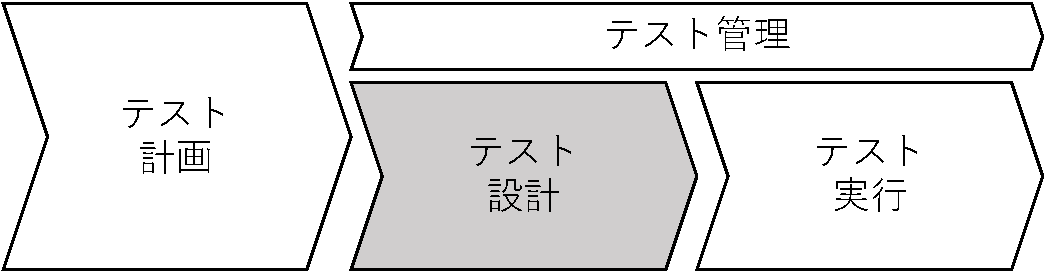
\includegraphics[clip,width=12cm]{test-task.pdf}
    \caption{テストにおけるタスク}
    \label{fig:1}
  \end{center}
\end{figure}

テスト工程は,表\ref{test-variety}のようにテスト対象の粒度によって単体テスト,結合テスト,システムテストの3種類に分類される.

\begin{table*}[t]
\caption{テストの種類}
\label{test-variety}
\begin{tabular}{|l|p{11cm}|}
\hline
\textbf{テスト粒度}                   & \textbf{説明}                                                                                                       \\ \hline
\textbf{単体テスト}        & プログラムを構成する比較的小さな単位の部品が個々の機能を正しく果たしているかどうかを検証するテスト \\ \hline
\textbf{結合テスト} & 個々の機能を果たすプログラムの部品(単体)を組み合わせて,仕様通り正しく動作するかを検証するテスト\\ \hline
\textbf{システムテスト}            & 個々の機能や仕組みを総合した全体像のシステムとして,仕様通り正しく動作するかを検証するテスト \\ \hline
\end{tabular}
\end{table*}

単体テスト設計タスクで作成されるテストケースは,テストプロセス,テスト入力値,テスト期待値から構成される.テストプロセスに従ってテスト対象のソフトウェアにテスト入力値を与え,その出力結果をテスト期待値と比較する.これが一致していればテストは合格となり,一致しなければ不合格となる.単体テスト設計タスクにおいては多くの場合,同値分割法,境界地分析法などのテストケース作成技法を用いてテスト入力値を作成するが,ソフトウェアの要求通りに動作するかを確認するために多くのバリエーションのテスト入力値を作成する必要がある.

\subsection{テストスメル}

テストスメルとは,テストコードの良くない実装を示す指標である.プロダクションコードの設計だけでなく,テストコードを適切に設計することの重要性は元々Beckら[]によって提唱された.さらに,Van Deursenら[50]は11種類のテストスメルのカタログ,すなわちテストコードの良くない設計を表す実装とそれらを除去するためのリファクタリング手法を定義した.このカタログはそれ以降,18個の新しいテストスメルを定義したMeszaros [42]によってより拡張された.

この節では,本研究で扱う以下の6種類のテストスメルを紹介する.

\begin{itemize}
\item Assertion Roulette
\item Default Test
\item Conditional Test Logic
\item Eager Test
\item Exception Handling
\item Mystery Guest
\end{itemize}

以降,それぞれのテストスメルについて説明する.

\begin{description}
\item[Assertion Roulette]~\\
Assertion Rouletteは,図\ref{AR}のようにテストメソッド内に複数のassert文が存在する場合発生する.各assert文は異なる条件をテストするが,開発者へ各assert文のエラーメッセージは提供されない,そのためassert文の1つが失敗した場合,失敗の原因を特定するが困難である.

\begin{figure}[htbp]
  \begin{center}
    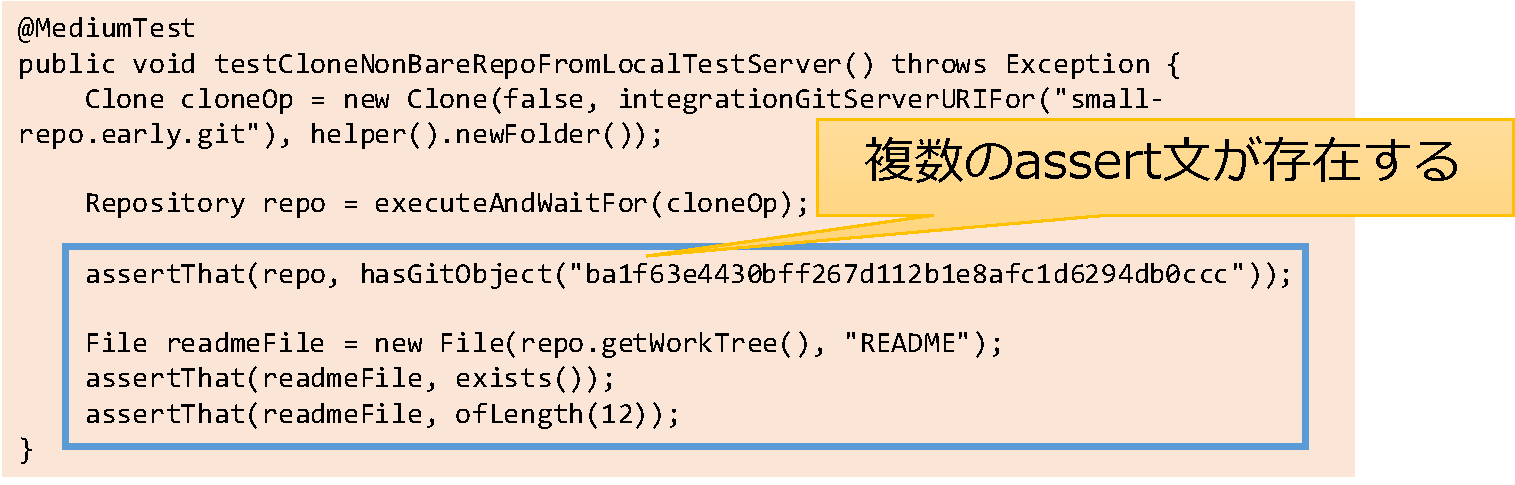
\includegraphics[clip,width=15cm]{AR.pdf}
    \caption{Assertion Rouletteの例}
    \label{AR}
  \end{center}
\end{figure}

\item[Default Test]~\\
Default Testは,図\ref{DT}のようにテストメソッド名が初期状態(意味のない名前)である場合発生する.テスティングフレームを使用した場合,クラス・メソッド名が初期状態である.テストコードの可読性向上のために適切な名前に変更する必要がある.

\begin{figure}[htbp]
  \begin{center}
    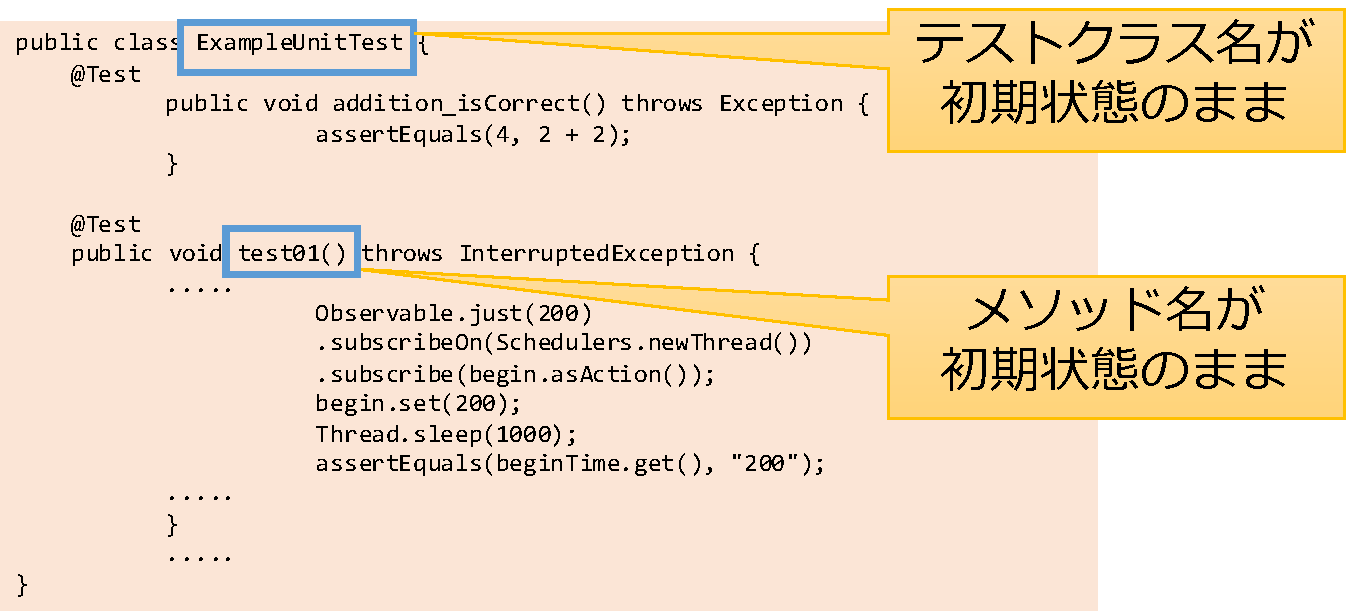
\includegraphics[clip,width=15cm]{DT.pdf}
    \caption{Default Testの例}
    \label{DT}
  \end{center}
\end{figure}

\newpage
\item[Conditional Test Logic]~\\
Conditional Test Logicは,テストメソッド内に複数の制御文が含まれている場合発生する(図\ref{CTL}).テストの成功・失敗は制御フロー内にあるassert文に基づくのでテスト結果を予測できない.また,条件分岐が多く複雑なテストコードは可読性を下げる.

\begin{figure}[htbp]
  \begin{center}
    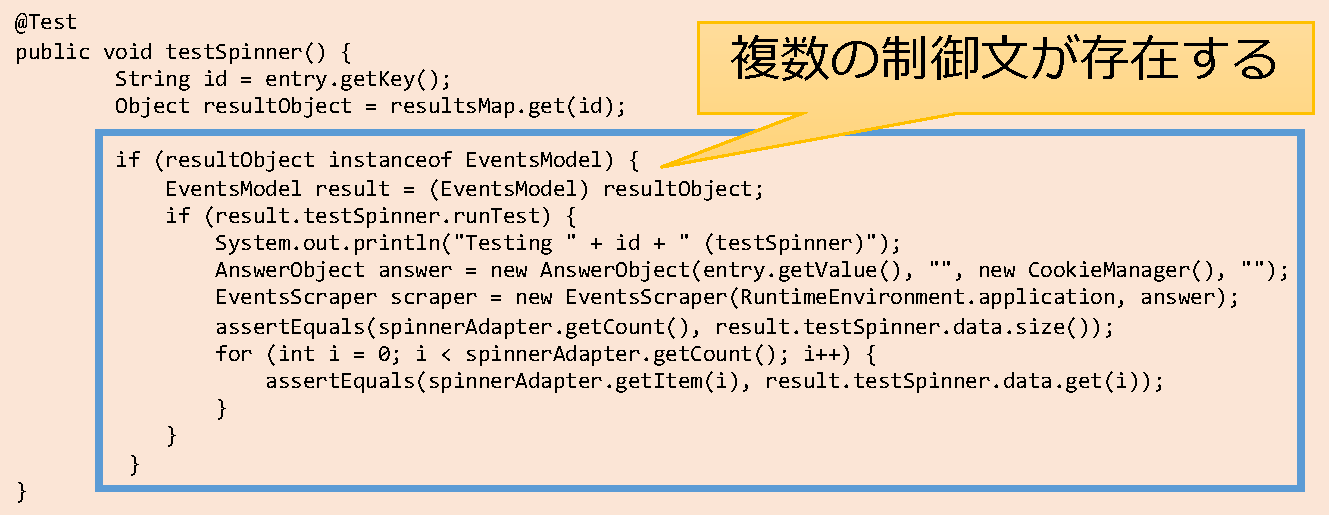
\includegraphics[clip,width=15cm]{CTL.pdf}
    \caption{Conditional Test Logicの例}
    \label{CTL}
  \end{center}
\end{figure}

\item[Eager Test]~\\
Eager Testは,テストメソッド内でテスト対象クラスのメソッドを複数回呼び出す場合発生する(図\ref{ET}).1つのテストメソッドで複数のメソッドを呼び出すと,他の開発者はどのテスト対象をテストするのか混乱が生じる.

\begin{figure}[htbp]
  \begin{center}
    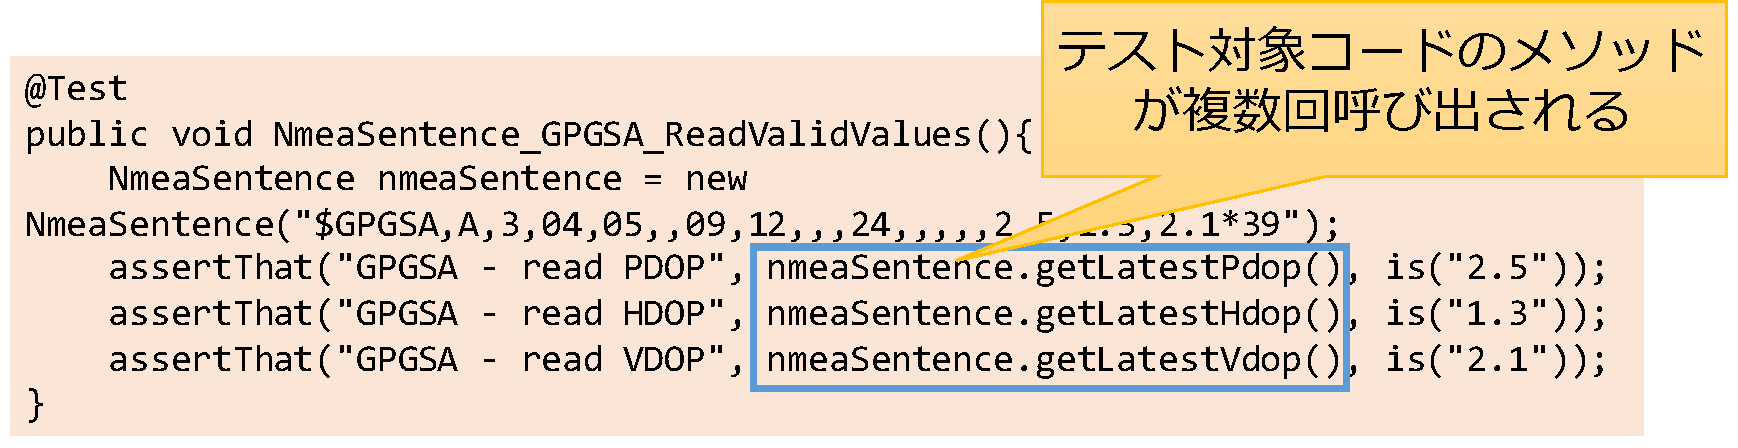
\includegraphics[clip,width=15cm]{ET.pdf}
    \caption{Eager Testの例}
    \label{ET}
  \end{center}
\end{figure}

\item[Exception Handling]~\\
Exception Handlingは,テストメソッド内に例外処理が含まれている場合発生する(図\ref{EH}).例外処理は,対象コードに記述すべきで,テストコード内では正しく例外処理が行われるかを確認すべきである.

\begin{figure}[htbp]
  \begin{center}
    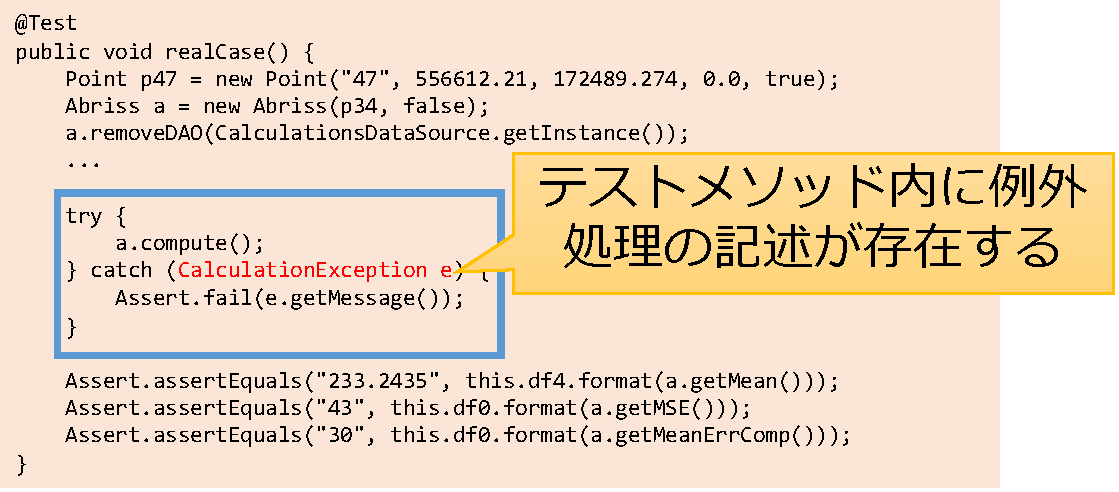
\includegraphics[clip,width=15cm]{EH.pdf}
    \caption{Exception Handlingの例}
    \label{EH}
  \end{center}
\end{figure}

\item[Mystery Guest]~\\
Mystery Guestは,図\ref{MG}のようにテストメソッド内で外部リソースを利用した場合発生する.テストメソッド内だけでなく外部ファイルなど,外部リソースを使用すると見えない依存関係が生じる.何らかの影響で外部ファイルを削除されるとテストが失敗してしまう.

\begin{figure}[htbp]
  \begin{center}
    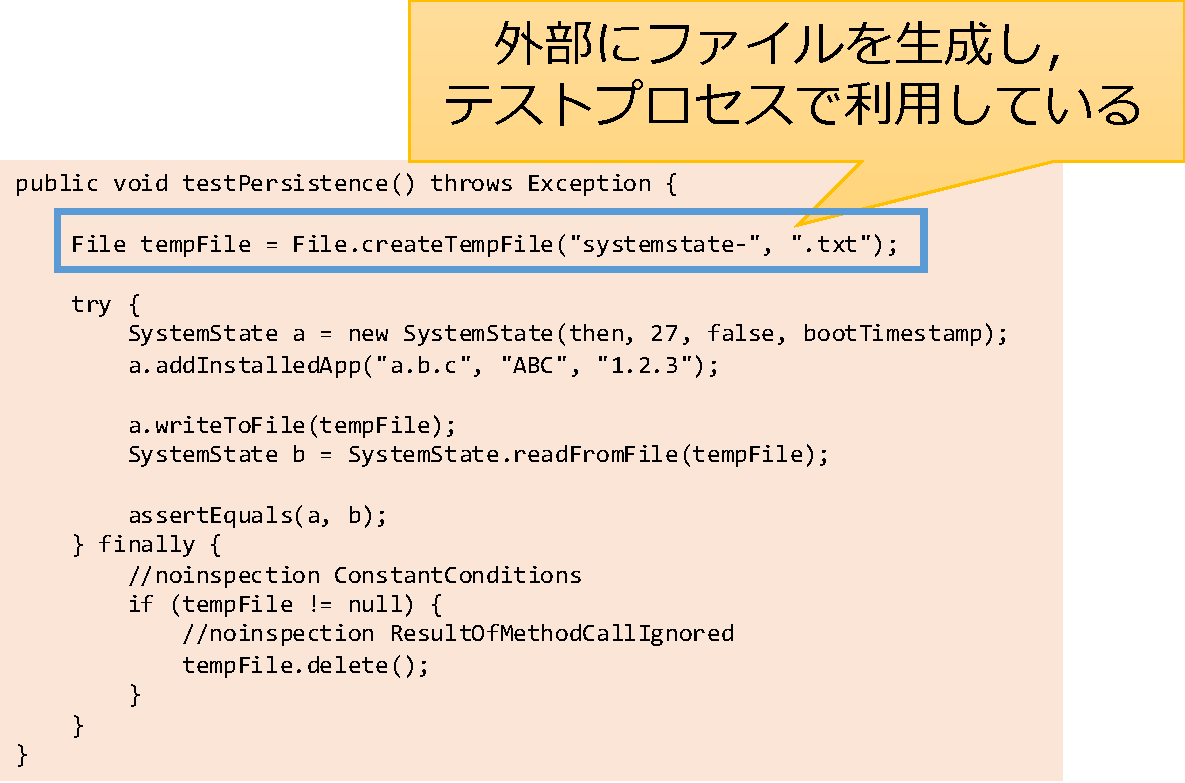
\includegraphics[clip,width=15cm]{MG.pdf}
    \caption{Mystery Guestの例}
    \label{MG}
  \end{center}
\end{figure}.
\end{description}

\begin{comment}
\subsubsection{Assertion Roulette}
Assertion Rouletteは,図\ref{AR}のようにテストメソッド内に複数のassert文が存在する場合発生する.各assert文は異なる条件をテストするが,開発者へ各assert文のエラーメッセージは提供されない,そのためassert文の1つが失敗した場合,失敗の原因を特定するが困難である.

\begin{figure}[htbp]
  \begin{center}
    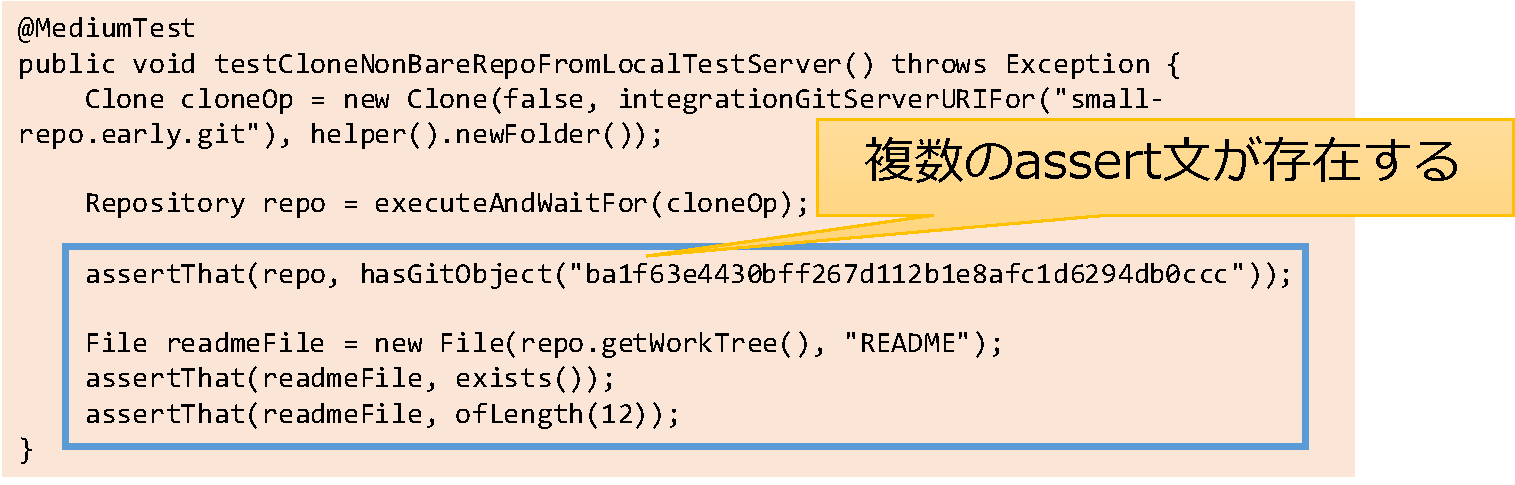
\includegraphics[clip,width=15cm]{AR.pdf}
    \caption{Assertion Rouletteの例}
    \label{AR}
  \end{center}
\end{figure}


\subsubsection{Default Test}

Default Testは,図\ref{DT}のようにテストメソッド名が初期状態(意味のない名前)である場合発生する.テスティングフレームを使用した場合,クラス・メソッド名が初期状態である.テストコードの可読性向上のために適切な名前に変更する必要がある.

\begin{figure}[htbp]
  \begin{center}
    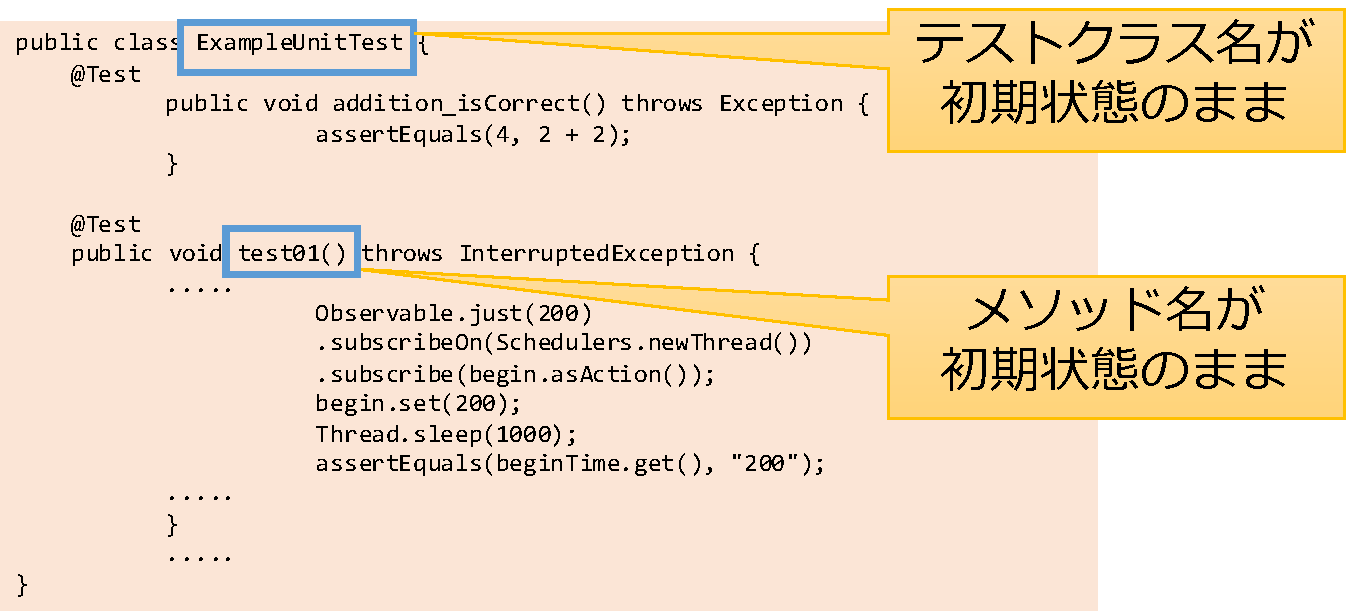
\includegraphics[clip,width=15cm]{DT.pdf}
    \caption{Default Testの例}
    \label{DT}
  \end{center}
\end{figure}

\subsubsection{Conditional Test Logic}
Conditional Test Logicは,テストメソッド内に複数の制御文が含まれている場合発生する(図\ref{CTL}).テストの成功・失敗は制御フロー内にあるassert文に基づくのでテスト結果を予測できない.また,条件分岐が多く複雑なテストコードは可読性を下げる.

\begin{figure}[htbp]
  \begin{center}
    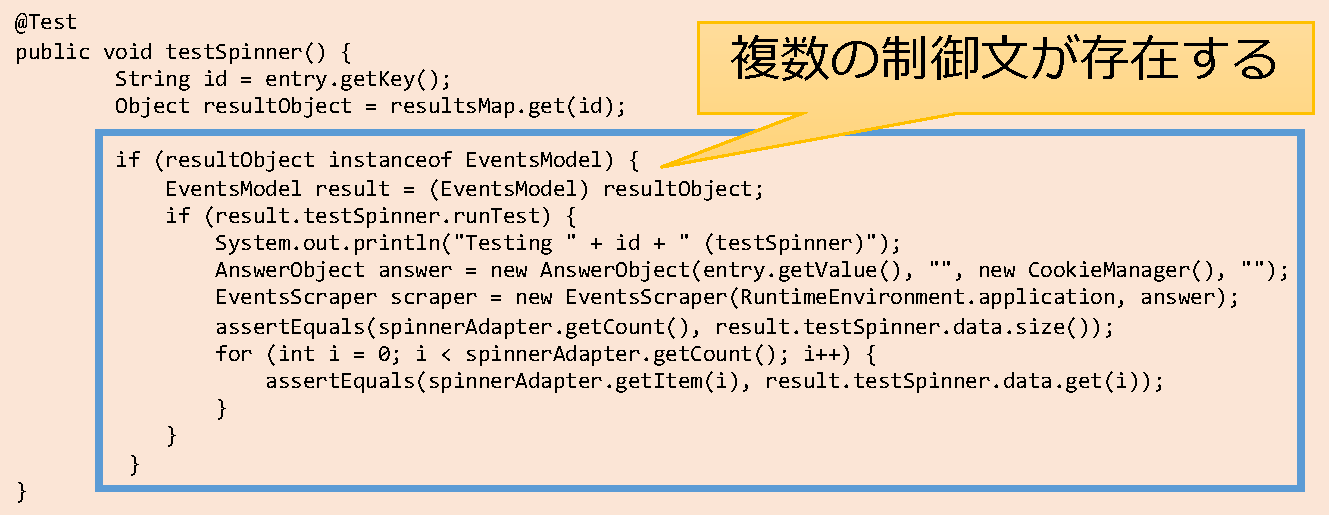
\includegraphics[clip,width=15cm]{CTL.pdf}
    \caption{Conditional Test Logicの例}
    \label{CTL}
  \end{center}
\end{figure}

\subsubsection{Eager Test}

Eager Testは,テストメソッド内でテスト対象クラスのメソッドを複数回呼び出す場合発生する(図\ref{ET}).1つのテストメソッドで複数のメソッドを呼び出すと,他の開発者はどのテスト対象をテストするのか混乱が生じる.

\begin{figure}[htbp]
  \begin{center}
    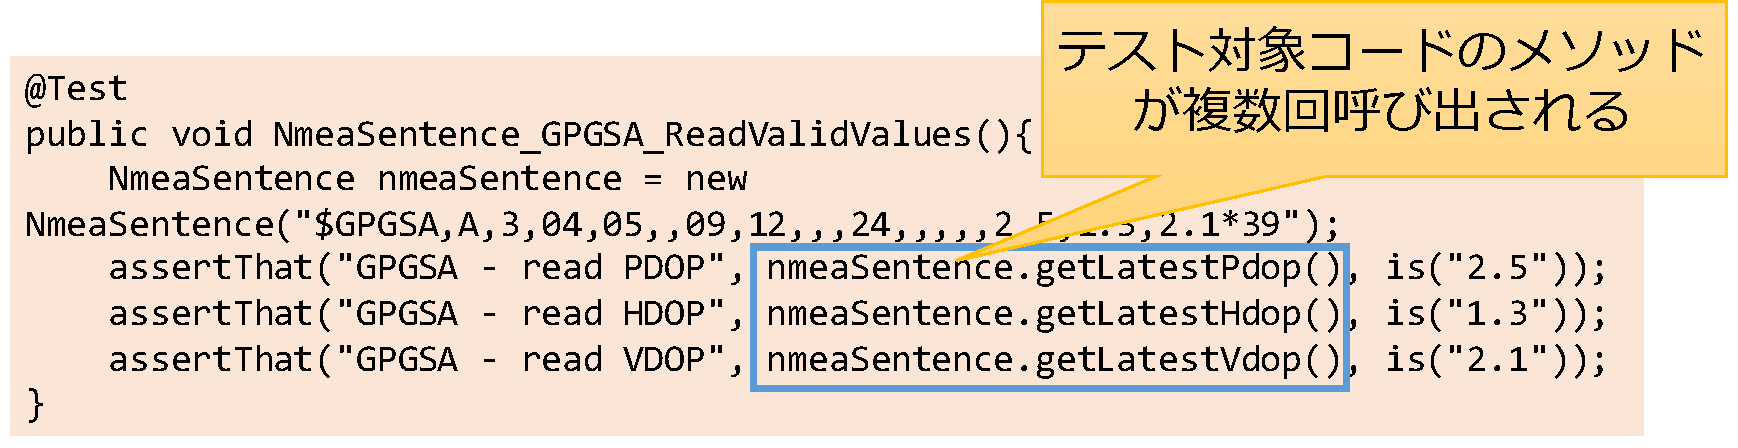
\includegraphics[clip,width=15cm]{ET.pdf}
    \caption{Eager Testの例}
    \label{ET}
  \end{center}
\end{figure}

\subsubsection{Exception Handling}

Exception Handlingは,テストメソッド内に例外処理が含まれている場合発生する(図\ref{EH}).例外処理は,対象コードに記述すべきで,テストコード内では正しく例外処理が行われるかを確認すべきである.

\begin{figure}[htbp]
  \begin{center}
    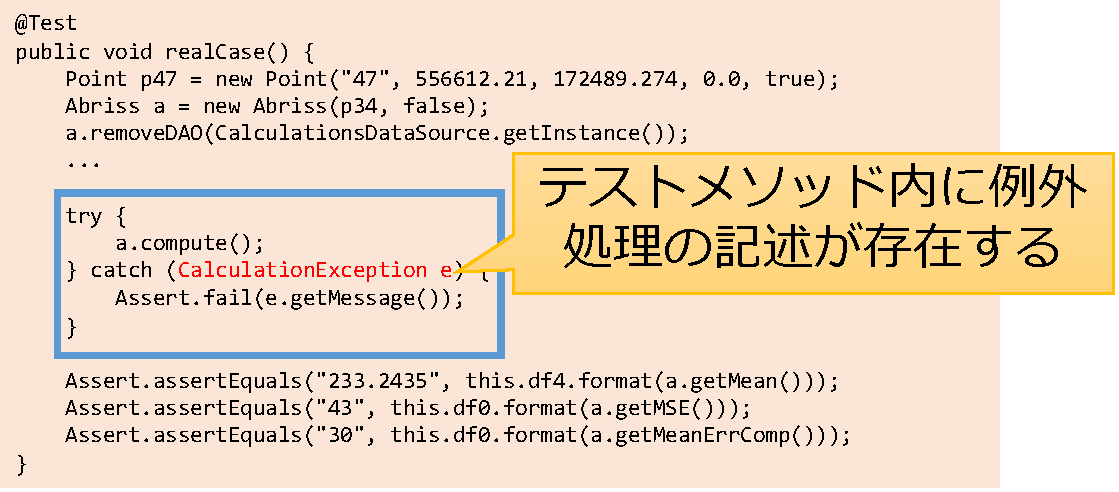
\includegraphics[clip,width=15cm]{EH.pdf}
    \caption{Exception Handlingの例}
    \label{EH}
  \end{center}
\end{figure}


\subsubsection{Mystery Guest}
Mystery Guestは,図\ref{MG}のようにテストメソッド内で外部リソースを利用した場合発生する.テストメソッド内だけでなく外部ファイルなど,外部リソースを使用すると見えない依存関係が生じる.何らかの影響で外部ファイルを削除されるとテストが失敗してしまう.

\begin{figure}[htbp]
  \begin{center}
    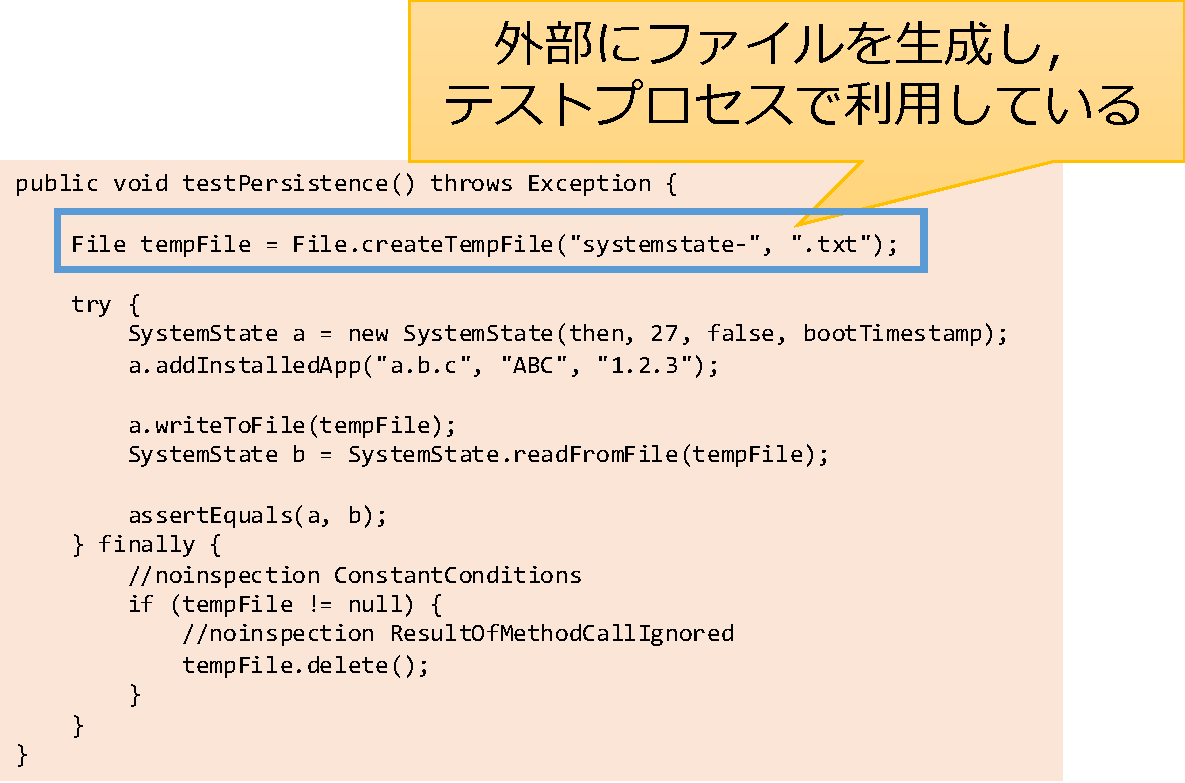
\includegraphics[clip,width=15cm]{MG.pdf}
    \caption{Mystery Guestの例}
    \label{MG}
  \end{center}
\end{figure}
\end{comment}

\subsection{テストスメルがソフトウェア保守にもたらす影響}

Bavotaら[7]は,18のソフトウェアプロジェクトにおけるテストスメルの拡散及びソフトウェアの保守に対するテストスメルの影響を調査した.調査結果は,JUnitクラスの82\%が少なくとも1つのテストスメルの影響を受けていること,さらにテストスメルの存在が影響を受けるクラスの理解に悪影響を及ぼすことを明らかにした.

Tufano[71]らは,ソフトウェアのライフサイクルにおけるテストスメルの重要性とその寿命を測定することを目的とした実証実験を行った.その結果,開発者はテストクラスに対して最初のコミットでテストスメルを導入し,およそ80\%のケースでテストスメルが除去されないことが分かった.

Davideら[]は,テストスメルが存在するテストコードは,そうでないテストコードと比べて変更が多く実施され,テスト対象コードは不具合を含んでいる可能性が高いことを示した.また,テストスメルの存在は開発者のテストコードの理解に悪影響を与えるだけでなく,テストコードがプロダクションコード内の不具合を見つけるのにあまり効果的でないと報告した.

Fabio Palomba[]らは,既存の自動生成ツールによって生成されるテストスイートは,プロジェクト内にテストスメルを拡散させることを確認した.生成されたJUnitクラス内83\%が少なくとも1つのテストスメルの影響を受けることを報告した.また,自動生成されたテストコード内ではAssertion Roulette,Eager Test,Test Code Duplicationの3つのテストスメルが多く検出される特徴があり,いくつかのテストスメルは同時に存在していることがすることを明らかにした.

自動生成ツールによって大量に生成されるテストスイートは,プロジェクト内にテストスメルを拡散させ開発者の可読性と保守性に大きな影響を与える可能性がある.一般にソフトウェアの保守にかかる継続的なコストは,テストコード作成コストをはるかに上回るため,初めに理解しやすく良質なテストコードを作成する必要がある.

\begin{comment}

\begin{table*}[t]
\caption{テストスメルの種類}
\label{testsmell-variety}
\begin{tabular}{|p{3cm}|p{11.5cm}|}
\hline
\textbf{テストスメル}                   & \textbf{説明}                                                                                                       \\ \hline
\textbf{Assertion Roulette}        & テストメソッド内に複数のassert文が存在する.各assert文は異なる条件をテストするが,開発者へ各assert文のエラーメッセージは提供されない,そのためassert文の1つが失敗した場合,失敗の原因を特定するが困難である. \\ \hline
\textbf{Default Test} & テストメソッド名が初期状態(意味のない名前)である.テスティングフレームを使用した場合,クラス・メソッド名が初期状態である.テストコードの可読性向上のために適切な名前に変更する必要がある.\\ \hline
\textbf{Conditional Test Logic}            & テストメソッド内に複数の制御文が含まれている.テストの成功・失敗は制御フロー内にあるassert文に基づくのでテスト結果を予測できない.また,条件分岐が多く複雑なテストコードは可読性を下げる. \\ \hline
\textbf{Eager Test}            & テスト対象クラスの複数のメソッドを呼び出す.1つのテストメソッドで複数のメソッドを呼び出すと,他の開発者は何をテストしているかについて混乱が生じる. \\ \hline
\textbf{Exception Handling}            & テストメソッド内に例外処理が含まれている.例外処理は,対象コードに記述すべきで,テストコード内では正しく例外処理が行われるかを確認すべきである. \\ \hline
\textbf{Mystery Guest}            & テストメソッド内で,外部リソースを利用する.テストメソッド内だけでなく外部ファイルなど,外部リソースを使用すると見えない依存関係が生じる.何らかの影響で外部ファイルを削除されるとテストが失敗してしまう. \\ \hline
\end{tabular}
\end{table*}

\end{comment}


\subsection{テストコード自動生成技術}
テスト工程の支援するために様々なテストコード自動生成技術が提案されている.既存の研究 [13] は,既存のテストケースを再利用,自動生成,または再適用することによって,ソフトウェア開発のテスト工程における時間とコストを大幅に節約できることを示している.テスト生成技術は,主にランダムテスト(RT),記号実行(SE),サーチベーステスト(SBST),モデルベース(MBT),組み合わせテストの5つに分類できる.SEはさらに静的記号実行(SSE)と動的記号実行(DSE)に分けられる.

既存研究で提案されているEvoSuite[]は,単体テスト自動生成における最先端のツールである.EvoSuiteは,SBSTを実装したツールであり,2011年に発表されて以来EvoSuiteをベースとした数多くの研究がなされており,大きな影響を与えている.SBSTでは,一般的に以下の手順でテストスイートを生成する.

\begin{enumerate}
  \item 達成したい要件に対する達成度合いを定量的に評価できる評価関数を設計
  \item 予め用意したテストスイートをテスト対象に対して実行し,実行したテストスイートの評価関数の値を取得
  \item 取得した評価関数の値が優れているテストスイートを元に,ヒューリスティック探索アルゴリズムによぅて新規にテストスイートを生成
  \item 3で生成したテストスイートをテスト対象に対して実行し,実行したテストスイートの評価関数の値を取得
  \item 設定した探索打ち切り条件を満たすまで,3,4を繰り返し実行
\end{enumerate}

評価関数の設計方法は,テスト実施の観点によって異なる.例えば,SBSTを用いてコードカバレッジ向上を目指したテストを実施する場合,評価関数は分岐網羅率等が用いられる.

SBSTを用いたテストケース自動生成の例を提示する.図\ref{SBST}において,SBSTを用いて分岐1で「$y > 1$」を満たすようなテスト入力値を生成したい場合,評価関数をプログラムが分岐1に到達したタイミングで評価する.このとき,$x$の値が大きいほど評価関数の値も大きくなり,「$y > 1$」を満たす度合いが大きくなると定量的に評価することができる.まず,$x = -10$として実行すると,評価関数の値は,$E = -10$となる.続いて,仮に$x = -5$として実行すると,評価関数の値は,$E = -5$となる.この場合,後者のテスト入力値の方が「$y > 1$」を達成するためには優れているテスト入力値,つまり$x$の値が大きいテスト入力値をベースに,新しいテスト入力値の生成が行われる.それにより徐々にxの値が大きいテスト入力値が生成されていき,最終的に$x = 1$等のテスト入力値が取得できる.

\begin{figure}[htbp]
  \begin{center}
    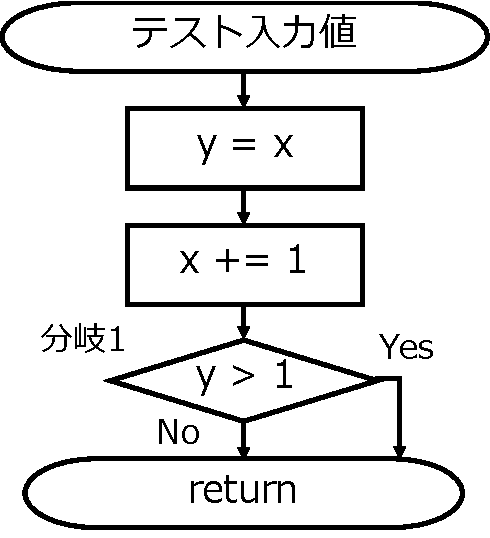
\includegraphics[clip,width=7cm]{SBST.pdf}
    \caption{SBSTによるテストケース生成の例}
    \label{SBST}
  \end{center}
\end{figure}

\subsection{既存の自動生成ツールにおける課題}

2.2節では,既存の単体テスト自動生成ツールEvoSuiteについて説明した.単体テストを自動生成することで,開発者は手作業でのテスト作成時間を節約することができ,またコードカバレッジを大幅に向上することができる.しかし,既存ツールによって自動生成されたテストコードは,対象コードの作成経緯や意図に基づいて生成されていないという性質から可読性が低く開発者に信用されていないことや後の保守作業を困難にするという課題がある [14], [15], [16].このことは,自動生成ツールの実用的な利用の価値に疑問を提示させる.テストが失敗するたびに,開発者はテスト対象のプログラム内で不具合の原因を特定するまたは,テスト自体を更新する必要があるかどうかを判断する必要がある.自動生成されたテストコードは,自動生成によって得られる時間の節約よりも読みづらく,保守作業に助けになるというよりかむしろ邪魔するという結果が報告されている [1].

我々は,この課題の解決するために既存テストの再利用が有効であると考える.本研究では,OSSに存在する既存の品質の高いテストコード推薦するツールを提案する.既存テストの利用はコーディング規約や命名規則に従った可読性の高いテストコードを利用できることや,人によって作成された信頼性の高いテストコードを利用できると考える.





\section{テストコード推薦手法}

本章では,本研究で提案するコードクローン検出技術を用いたテストコード自動推薦ツール{\sf SuiteRec}について述べる.本研究では,コードクローン検出技術を利用し,オープンソースソフトウェア(以下,OSS)上に存在する既存の高品質なテストコード推薦することで,開発者のテストコード作成を支援することが目的である.{\sf SuiteRec}の基となるアイディアは,クローンペア間でのテストコード再利用である.{\sf SuiteRec}は,開発者からの関数単位の入力コード対してその類似コード片を検出する.そして,類似コード片に対応するテストスイートを開発者に推薦する.さらに,推薦されるテストコード内に含まれるテストスメルを提示し,より品質が高いテストスイートを推薦できるように推薦順位がランキングされる.

図\ref{SO}は,SuiteRecによってテストスイートが推薦されるまでの流れを示す.推薦手法は,主に以下の4つのステップから構成される.

\begin{figure}[htbp]
  \begin{center}
    \includegraphics[clip,width=15cm]{SuiteRec-outline.pdf}
    \caption{提案手法の概要}
    \label{SO}
  \end{center}
\end{figure}

\begin{description}
\item[Step1]~\\
{\sf SuiteRec}は,開発者から入力コードを受け取ると,既存のコードクローン検出ツールを用いて,入力コードに対応する類似コードを検出する.
\item[Step2]~\\
複数の類似コードが検出されると,次にその類似コードに対応するテストスイートをテストコードデータベース内から検索する.
\item[Step3]~\\
各類似コードのテストスイートが検出されると,次にそれらをテストスメル検出ツールにかけ各テストスイートに含まれるテストスメルを検出する.
\item[Step4]~\\
最後に,Step1で得られた類似コードと入力コードの類似度とStep3で検出されたテストスメルの数を基に出力されるテストスイートの順番がランキングされる.
\end{description}

以降の節で,それぞれのステップの詳細について説明する.

\subsection{Step1: 類似コード検出}

Step1では,開発者から受け取った関数単位のコード片に対して類似コードを検出する.本研究では,コードクローン検出ツールとして{\sf NiCad}\cite{b2}を採用した.{\sf NiCad}は検出対象のコード片のレイアウトを統一的に変換させ,行単位で関数単位のコード片を比較することで,クローンペア検出するツールであり,このような手法を取ることで,高精度・高再現率でのクローンペアの検出を実現している.

本研究で,{\sf NiCad}を採用した理由として以下の2点が挙げられる.

\begin{itemize}
\item 単体テストの再利用を考える上で関数単位のコード片を高精度で検出できる
\item 構文的に類似したtype2,type3のコードクローンを高速に検出できる
\end{itemize}


{\sf NiCad}は,プロジェクトを入力とし,プロジェクト内のコードクローンをすべて検出する.検出されるコードクローンはクローンクラスとして出力される.{\sf SuiteRec}は,{\sf NiCad}の検出結果の中で入力コードを含むクローンクラスを特定し,そのクローンクラスに含まれるコード片をすべて類似コードとして扱う.

{\sf SuiteRec}は,{\sf NiCad}を用いて入力コード対応する類似コードを大規模なOSSプロジェクトを保持するGithubのリポジトリから検索する.図\ref{SO}のソースコードデータベースは,テストコードが存在するGithub上の3,205プロジェクトのプロダクションコードが格納されている.具体的には,プロジェクト内にテストフォルダが存在し,JUnitのテスティングフレームワークを採用しているプロジェクトを選択した.

{\sf NiCad}は,一度に検索できるプロジェクトの規模限度がある.我々は,検索時間を短縮するために大規模なプロジェクトは分割し,小規模なプロジェクトは統合させた状態で検索処理を複数並列して走らせることで現実的な時間での類似コードの検索を実現した.また,検出設定については{\sf NiCad}の標準設定で提案ツールに実装した.

\subsection{Step2: テストコードの検索}
Step2では,Step1で検出された類似コード片に対応するテストコードを検索する.大規模なプロジェクトのテストコードが格納されているテストコードデータベース(以下,TDB)からテストコードを検出ために,テスト対象コードとテストコードの対応付けを行う.

本研究では,対象コードとテストコードを対応付けるために以下の3つのステップを実施する.

\begin{enumerate}
  \item 命名規則によるクラス単位での対応付け
  \item テストコードを静的解析し,各テストケースから呼び出されるすべてのメソッド名を収集する
  \item テストメソッド名を区切り文字や大文字で分割し,対象メソッドと部分一致した場合,テストコードと対象コードをメソッド単位で対応付ける
\end{enumerate}

本研究では,テストコードとしてJUnitテスティングフレームワークを用いた単体テストを対象とする.Step1では,JUnitの命名規則に従ってテストクラス名の先頭または,末尾に``Test''という文字列が含まれるテストクラスを収集し,収集したテストクラスから``Test''を除いたクラス名をテスト対象クラスとする.例えば,CalculatorクラスとCalculatorTestクラスが対応付けられる.

Step2では,テストコードを静的解析し,テストメソッド内で呼び出されるメソッド名を取得する.単体テストでは,図\ref{fig2}の例のようにテストコード内でオブジェクトの生成が行い,テスト対象コードのメソッド呼び出して実行される.すなわち,テストコードリポジトリ内のテストコードを静的解析し,メソッド呼び出しを取得することで,テスト対象コードとテストコードを対応付ける.しかし,テストメソッド内では複数のメソッドが呼び出されていることも考えられるのでStep3ではさらに,メソッド名の比較も行う.テストメソッド名の記述方法としてテスト対象メソッドの処理の内容を忠実に表すことが推奨されており,対象メソッドの名前が記述されていることが多い\cite{b22}.したがって,テストメソッドの名前を区切り文字や大文字で分割し,対象メソッドと部分一致した場合,対応付けるように実装した.

\begin{figure}[htbp]
  \begin{center}
    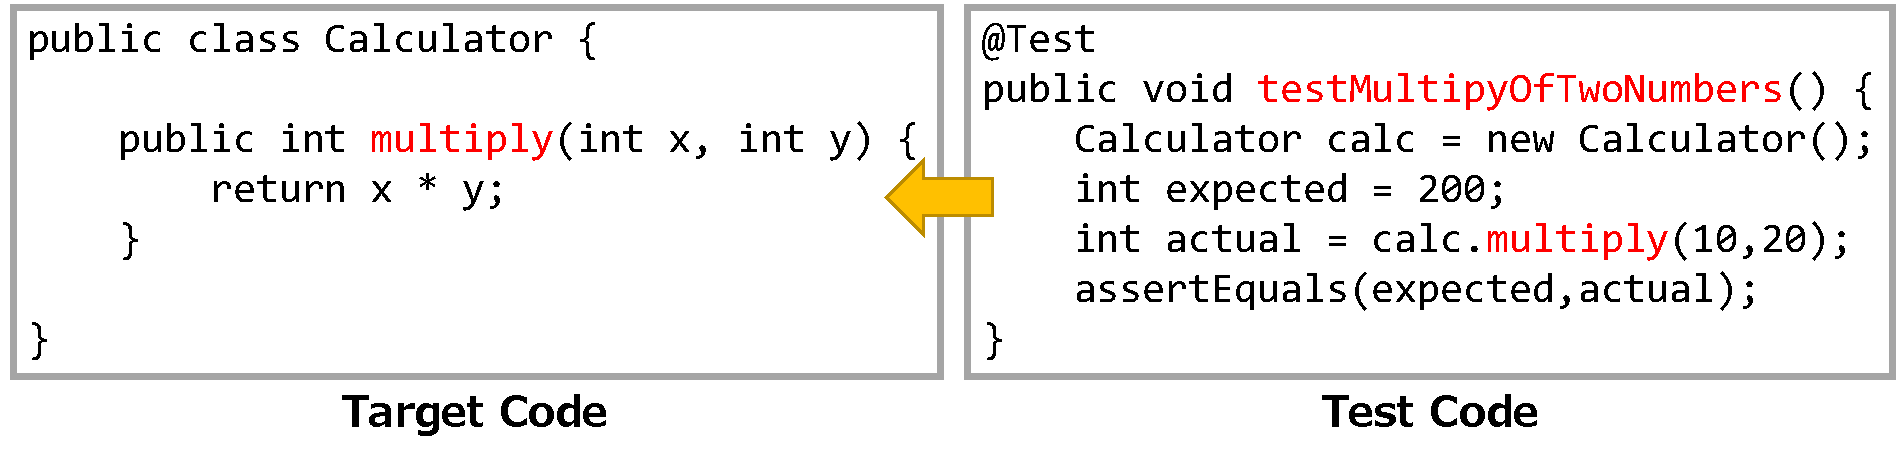
\includegraphics[clip,width=15cm]{mapping.pdf}
    \caption{テストコードと対象コードの対応付け}
    \label{map}
  \end{center}
\end{figure}

\subsection{Step3: テストスメルの検出}

Step3では,Step2で検索されたテストスイート内のテストスメルを検出する.本研究では,テストスメル検出ツールとして{\sf tsDetect}\cite{b10}を採用した.{\sf tsDetect}はASTベースの検出手法で実装されたツールであり,19種類のテストスメルを検出できるツールである.また,85\%〜100\%の精度と90\%〜100\%の再現率でテストスメルを正しく検出でき,多くの研究で利用されている[][][].本研究では,{\sf tsDetect}で検出できる19種類のテストスメルの内,2.4節で説明したテストコードの推薦を考える上で重要な6種類のテストスメルを提示するように実装した\cite{b9}.

{\sf tsDetect}は,ASTベースの検出手法であり大規模なテストコードに対して実行すると計算コストが高い.我々は,事前にTDB内のテストコードのテストスメルを検出しその情報をテストコードに対応付けてTDBに格納した.これにより,推薦プロセスにおけるテストスメル検出時間を短縮化した.また,推薦テストコードとして相応しくない以下の4つのテストスメルを含むテストコードを事前にTDBから除去し,推薦されるテストコードとして出力されないようにした.

\begin{itemize}
\item \textbf{Empty Test.}テストメソッド内にテストの記述はなくコメントのみが含まれているテストコード
\item \textbf{Ignored Test.}@Ignoreアノテーションがあり,実行されないテストコード
\item \textbf{Redundant Assertion.}必ずテストが成功する意味のないテストコード
\item \textbf{Unknow Test.}assert文が存在しないテストコード
\end{itemize}

\subsection{Step4: 推薦されるテストコードのランキング}

最後のStep4では,推薦されるテストスイートをランキングし,開発者が求める順番でテストスイートを提示する.

SuiteRecのランキングは,Step1の入力コード片と類似コード片の類似度とStep3で検出されたテストスメルの数を基に計算する.我々は,以前の調査[fose2019]で,クローンペア間とテストコードの類似度の関係を調査した.詳細には,OSS上に存在する3つの有名Javaプロジェクト内にある両方のコード片にテストコードが存在するコードクローンを対象に,クローンペア間の類似度とそれぞれのコード片に対応するテストコードの類似度を関係を調査した.その結果,テストコードの間の類似度と対象のクローンペア間の類似度には相関関係があり,クローンペア間の類似度が高いほどテストコードを再利用できる可能性が高いことが分かっている.SuiteRecではこの結果を基に類似度が高いクローンペアの順に並び替え,さらに類似度が同じ場合,テストスメルの数で順番を決定するように推薦ランキングを実装した.

本研究では,クローンペア間の類似度をNiCadで用いられる計算方法{\it Unique Percentage of Items}(以下,UPI)を利用して計算する.以下に,UPIの計算式を示す.

\[
  Unique\, Percentage\, of\, Items\, (UPI) =
  \frac{No.\, of\, Unique\, Items * 100}{Total\, No.\, of\, Items}
\]

ここで,{\it No.of Unique Items}は,入力コード片と類似コード片を行単位で比較した際に一致した行の数を意味する.{\it Total No.of Items}は,コード片内のすべての行の数を意味する.比較対象のコード片の{\it Total No.of Items}が異なる場合,行数が大きい方の{\it Total No.of Items}を用いて計算する.例えば,入力コード片の行数が10,類似コード片の行数が12で,一致した行数が9の場合,入力コード片と類似コード片の類似度は75\%になる.


\begin{figure}[htbp]
  \begin{center}
    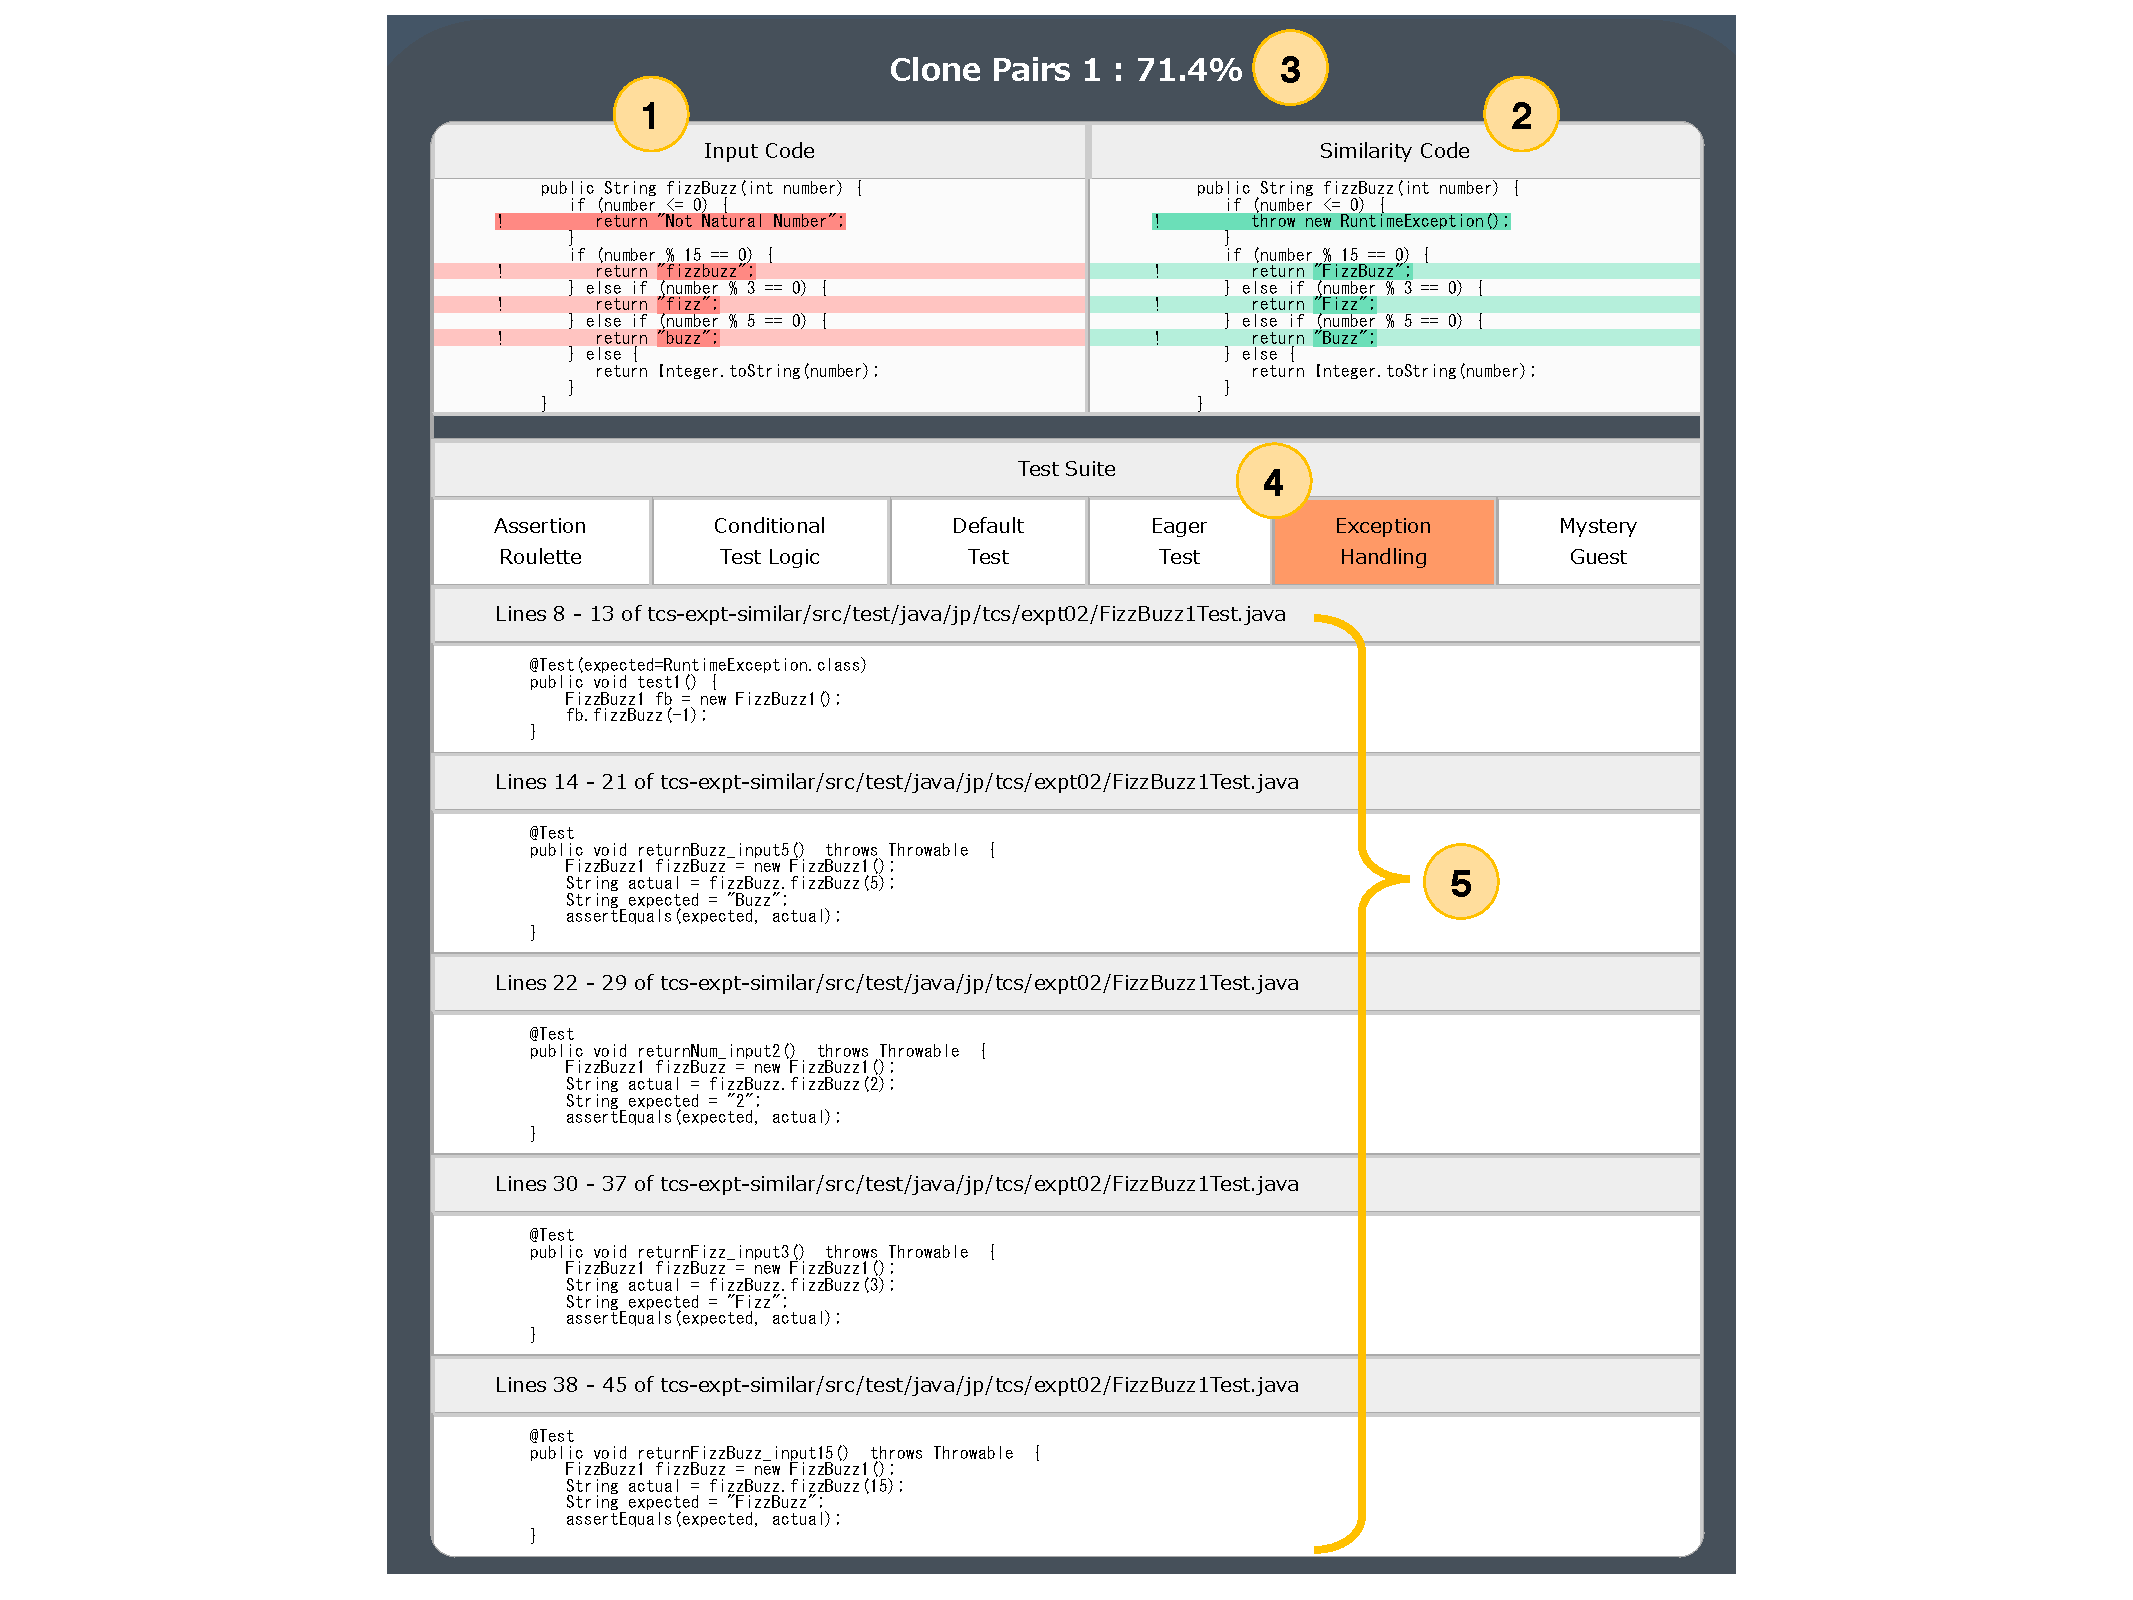
\includegraphics[clip,width=15cm]{SuiteRec.pdf}
    \caption{SuiteRecから推薦されるテストコード}
    \label{SR}
  \end{center}
\end{figure}

図\ref{SR}は{\sf SuiteRec}から推薦されるテストコードの例である.以下に{\sf SuiteRec}のインターフェースについて各項目の説明を示す.

\newpage
 \begin{enumerate}
\renewcommand{\labelenumi}{(\arabic{enumi})}
\item{\textbf{Input Code Fragment.}開発者が入力した関数単位のプロダクションコードが表示される.}
\item{\textbf{Similarity Code Fragment.}入力コードに対する類似コードが表示される.入力コードと類似度コードの違いが分かるように差分がハイライトされる.}
\item{\textbf{Degree of similarity.}入力コードと類似コードの類似度が表示される.類似度はNICADで用いられている計算方法Unique Percentage of Items(UPI)を採用した.}
\item{\textbf{Test Smells.}推薦されるテストスイート内にテストスメルが含まれている場合,そのテストスメルがオレンジ色にハイライトされ開発者にテストスメルの存在を提示する.}
\item{\textbf{Recommend Test Suites.}推薦されるテストスイートが表示される.また,どのプロジェクトからテストコードが参照されたのかを示すためにファイルパスも表示される.}
\end{enumerate}

\section{評価実験}
この章では,SuiteRecを定量的及び定性的に評価するために,被験者による実験を行う.実験では,被験者に3つのプロダクションコードのテストコードを作成してもらい,SuiteRecを使用して作成した場合とそうでない場合のテストコードを比較することで評価を行う.実験を通してコードカバレッジ,実験タスクを終了するまでの時間およびテストコードの品質に関するデータを収集することで,以下のリサーチクエスチョンに答えることを目指す.

\begin{description}
\item[\textbf{RQ1: {\sf SuiteRec}は高いカバレッジを持つテストコードの作成を支援できるか?}]~\\
RQ1では,被験者が作成したテストコードのカバレッジを測定する.テスト工程において,ソフトウェアの品質を確認する1つの指標としてカバレッジは重要な要素である.テストコード内で一度も実行されない行が存在するとその部分の品質を確保することはできない.SuiteRecの利用は高いカバレッジを達成するために役に立つのか?
\item[\textbf{RQ2: {\sf SuiteRec}はテストコードの作成時間を削減できるか?}]~\\
RQ2では,被験者のテストコード作成タスクに費やす時間を測定する.開発者はSuiteRecで推薦されるテストコードを参考にすることで,テストコード作成時間を短縮化できるのか?
\item[\textbf{RQ3: {\sf SuiteRec}は,高い品質を持つテストコードの作成を支援できるか?}]~\\
RQ3では,被験者が作成したテストコード内に含まれるテストスメルを検出し,テストコードの品質を測定する.開発者はSuiteRecで推薦されるテストコードを参考にすることで,品質の高いテストコードを作成することができるのか?
\item[\textbf{RQ4: {\sf SuiteRec}の利用は,開発者のテストコード作成タスクの認識にどう影響するか?}]~\\
RQ4では,テストコード作成タスクを完了した被験者に作成タスクに関するアンケート回答してもらった.SuiteRecを利用した場合,テストコードの作成が容易になり,自身で作成したテストコードに自信が持てるのか?
\item[\textbf{RQ5: {\sf SuiteRec}は,開発者が求める順番でテストスイートをランキングできるか?}]~\\
RQ5では,SuiteRecから推薦されるテストスイートのランキングの妥当性を検証する.
\end{description}

以降,4.1節では,本実験に参加した被験者について説明する.4.2節では,被験者に実施してもらう実験タスクについて説明する.最後に4.3節で,実験手順について説明する.

\subsection{被験者の選択}
\subsection{実験タスクの作成}
\subsection{実験手順}


\begin{comment}

\subsection{過去における研究}
\label{kako}


\subsection{研究の目的と意義}


\begin{figure}
\centerline{ここに図を書く}
\caption{これは図の例}
\end{figure}

\begin{table}
\centerline{ここに表を書く}
\caption{これは表の例}
\end{table}




\newpage




\newpage
\section{現状と今後の課題}
\label{kadai}



%
% 謝辞
%
\acknowledgements

Thank you. Thank you.
%
% 参考文献
% ここでは \reference を使って、自分でリストを作るか、BibTeX を使って
% リストをつくって下さい。この例では BibTeX を作るような形式になってい
% ます。
%
\newpage
% \reference
\bibliographystyle{plain}
\bibliography{mthesis}
%
% 付録
%
\appendix

\section{おまけその1}
\label{omake1}



\begin{figure}
\centerline{これはおまけの図です。}
\caption{おまけの図}
\end{figure}


\section{おまけその2}

\end{comment}

\end{document}

